
\begin{figure}[htb]
  \centering
  \begin{tabular}{c c c c c }
    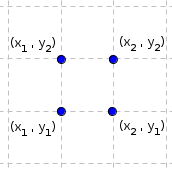
\includegraphics[width=3.5cm]{./img/dispositionFrameInGrid}    
    & &
   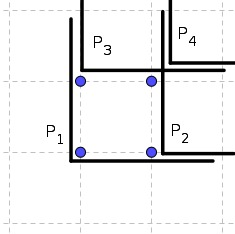
\includegraphics[width=3.5cm]{./img/frame2} 
     & &
   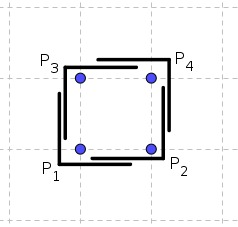
\includegraphics[width=3.5cm]{./img/square2} \\%[\abovecaptionskip]
   {\footnotesize (a) Coordinates of bends of a frame}  
   & & {\footnotesize (b) An example of a frame} 
   & & {\footnotesize (c) A square-frame} %\label{fig:frame}
  \end{tabular}
  \caption{$B_{1}$-EPG representation of the induced cycle of size 4 as frame}\label{fig:frameInGrid}
\end{figure} 
